\chapter{IMPLEMENTASI}
Tahap implementasi pada penelitian ini menggunakan memiliki beberapa tahap yang terbagi menjadi empat yaitu \textit{data collection}, \textit{data labelling}, \textit{training}, \textit{testing}.
Data collection pada penelitian ini adalah proses pengumpulan dataset yang dilakukan dengan melakukan akuisisi citra menggunakan webcam dan pengunduhan dataset \textit{public}. Data yang di dapatkan dari proses akuisisi citra akan dilakukan \textit{preprocessing} terlebih dahulu sebelum dilakukan proses labelling sesuai dengan klasifikasi. Tahap \textit{training} digunakan untuk ekstraksi fitur dataset yang disimpan dalam sebuah model. Model yang terbentuk akan dilakukan proses pengujian pada tahap testing.

\section{Data Collection}
Data yang digunakan dalam penelitian ini adalah data yang diampbil dari proses akuisisi citra dan dataset \textit{American Sign Language} dari \textit{Massey University}. Dataset yang diambil dari proses akuisisi citra sebanyak 1000 citra tangan yang diambil dari 10 orang. Selanjutnya untuk dataset \textit{American Sign Language} akan dilakukan preprocessing terlebih dahulu sebelum dijadikan format csv yang berisi nama dan lokasi citra.

\subsection{Implementasi Proses Akuisisi Citra}
Tahap akuisisi citra dilakukan bertujuan mendapatkan dataset untuk deteksi objek tangan sehingga dataset yang diambil adalah pose tangan dari subjek. Setiap subjek akan diambil sebanyak 100 citra sehingga menghasilkan 1000 citra. Pada program yang dibuat akan melakukan penyimpanan citra pada folder tertentu dengan setiap nama masing masing subjek. Gambar 5.1 menunjukan kode implementasi saat proses akuisisi citra berlangsung.
\begin{figure}[H]
	\centering
	\lstinputlisting[language=python]{collect-data-object-detection.py}
	\caption{Source code akuisisi citra}
\end{figure}

\subsection{Implementasi Data Augmentasi}
Proses augmentasi data digunakan untuk menduplikat citra dengan variasi yang berbeda. Pada proses augmentasi ini diterapkan untuk dataset \textit{American Sign Language} karena hanya memiliki 700 citra untuk 10 klasifikasi. Sebelum dilakukan augmentasi, citra pada dataset \textit{American Sign Language} akan dilakukan \textit{resize} pada ukuran (224x224). Augmentasi yang dilakukan berupa variasi intensitas cahaya, intensitas warna, operasi morfologi, \textit{filtering} dan rotasi.
% TODO: \usepackage{graphicx} required
\begin{figure}[H]
	\centering
	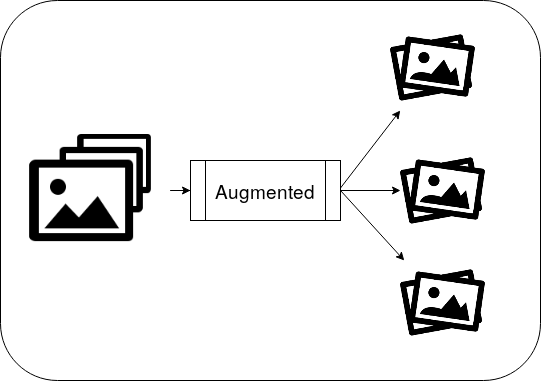
\includegraphics[width=0.6\linewidth]{augmented}
	\caption{Implementasi Augmentasi}
	\label{fig:augmented}
\end{figure}

Citra dataset dengan total 700 citra akan diaugmentasi 17 kali dengan beberapa filter dan transformasi yang berbeda-beda untuk setiap citra. Citra hasil augmentasi sejumlah 11900 citra kemudian ditambah dengan 700 citra dataset, sehingga total citra yang akan di training menjadi 12600 untuk 10 klasifikasi.
\begin{figure}[H]
	\centering
	\lstinputlisting[language=python]{augmen.py}
	\caption{Source Code Augmentasi Citra}
\end{figure}
\subsection{Pembuatan file CSV}
Dataset dari pengenalan gestur akan dibuat file CSV yang berisi label dan lokasi dari setiap citra dalam dataset. Fungsi tocsv berikut adalah implementasi dari pembuatan file CSV
\begin{figure}[H]
	\centering
	\lstinputlisting[language=python]{csv.py}
	\caption{Source Code Pembuatan file CSV}
\end{figure}
Hasil dari implementasi csv tersebut akan digunakan untuk refrensi input dalam proses pelatihan pengenalan gestur. Berikut adalah hasil dari pembuatan file csv dataset.
% TODO: \usepackage{graphicx} required
\begin{figure}[H]
	\centering
	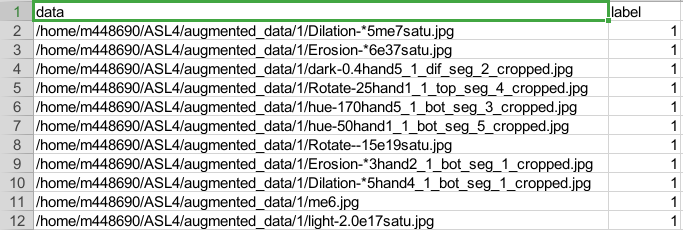
\includegraphics[width=0.7\linewidth]{csv}
	\caption{Hasil File CSV}
	\label{fig:csv}
\end{figure}
\section{Implementasi Data Labelling}
Pelabelan sebuah citra dilakukan untuk memberikan pengenalan suatu objek yang ada dalam sebuah citra, pada proses pelabelan menyimpan anotasi yang berisi informasi gambar yang disimpan dalam file XML yang berformat PASCAL VOC. Setiap data dilakukan pelabelan sesuai dengan nama objek yang mau di deteksi dalam hal ini adalah tangan yang diberi label \textit{hand}. Proses pelabelan ditunjukan pada gambar xxxx.
% TODO: \usepackage{graphicx} required
\begin{figure}[H]
	\centering
	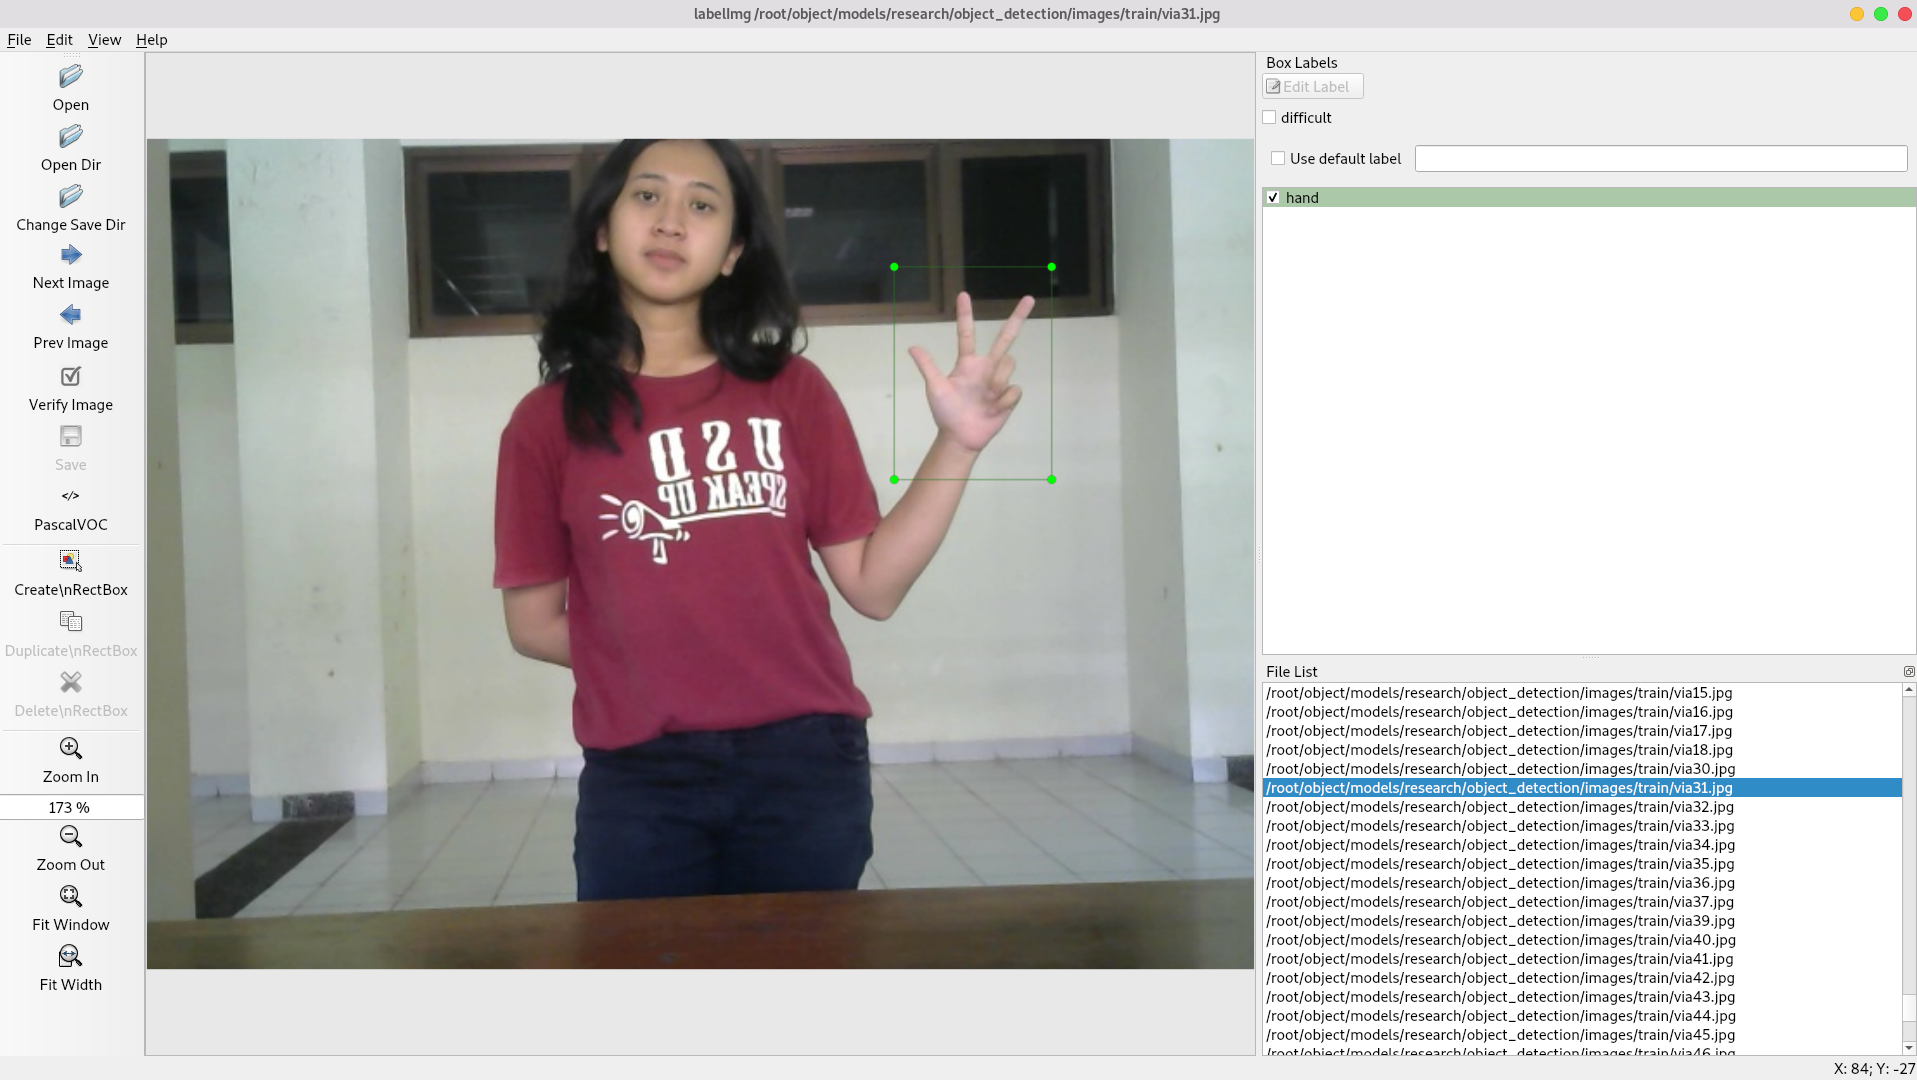
\includegraphics[width=0.8\linewidth]{viany}
	\caption{Proses Pelabelan Citra}
	\label{fig:viany}
\end{figure}
Hasil citra terlabel dijadikan refrensi dalam informasi XML atau anotasi dari citra tertentu. berikut adalah contoh hasil anotasi dari salah satu citra.
% TODO: \usepackage{graphicx} required
\begin{figure}[H]
	\centering
	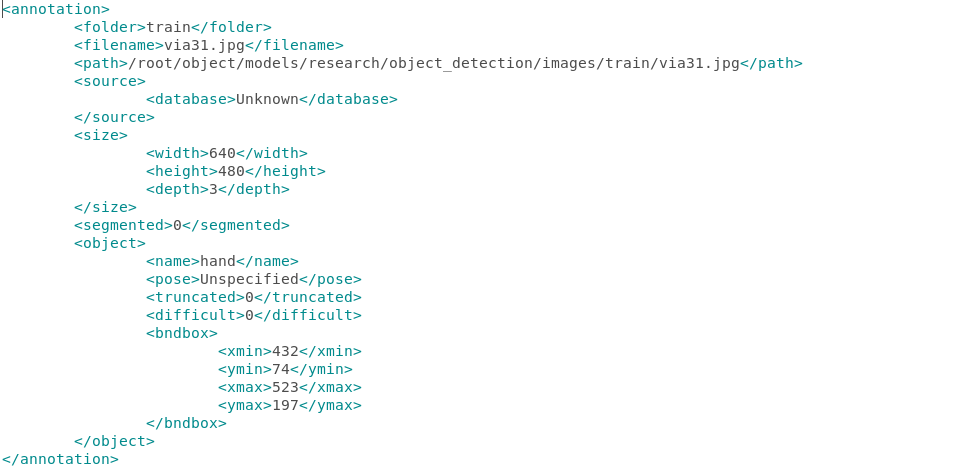
\includegraphics[width=0.8\linewidth]{anotasi}
	\caption{hasil anotasi citra}
	\label{fig:anotasi}
\end{figure}
\section{Implementasi Pembuatan TFRecord file}
Proses selanjutnya adalah mengubah informasi XML ke CSV dengan tujuan membuat format \textit{Tensorflow} dataset atau \textit{TFRecord}. Berikut program konversi file dataset.
\begin{figure}[H]
	\centering
	\lstinputlisting[language=python]{xml.py}
	\caption{Source Code Pengubahan XML ke CSV}
\end{figure}
\begin{figure}[H]
	\centering
	\lstinputlisting[language=python,lastline=30]{tfrecord.py}
\end{figure}
\begin{figure}[H]
	\centering
	\lstinputlisting[language=python,firstline=31,firstnumber=31]{tfrecord.py}
	\caption{Source Code Pembentukan TFRecord}
\end{figure}
\section{Konfigurasi \textit{Pipeline Object Detection}}
Proses pelatihan Tensorflow Object Detection API  menggunakan konfigurasi pipeline, beberapa konfigurasi tersebut diantaranya model, training\_config, eval\_config, train\_input\_config, eval\_input\_config. Dataset yang berformat \textit{TFRecord akan di lewatkan sebagai input} dan model pada \textit{ssd mobilenet v2} akan digunakan sebagai \textit{pretrained} model. Berikut adalah konfigurasi yang digunakan
\begin{figure}[H]
	\centering
	\lstinputlisting[language=python,firstline=177,lastline=196]{ssd_mobilenet_v2_fpnlite_640x640_coco17_tpu-8.config}
\end{figure}
\begin{figure}[H]
	\centering
	\lstinputlisting[language=python,firstline=142,lastline=175,firstnumber=20]{ssd_mobilenet_v2_fpnlite_640x640_coco17_tpu-8.config}
	\caption{konfigurasi pipeline \textit{Object Detection}}
\end{figure}
\section{Implementasi Training}
\subsection{Object Detection}
Tahap pelatihan dalam \textit{object detection} menggunakan arsitektur mobilenet v2, proses pelatihan berlangsung dengan menggunakan parameter pada konfigurasi pipeline. berikut adalah program untuk melakukan pelatihan.
\begin{figure}[H]
	\centering
	\lstinputlisting[language=python,firstline=37,lastline=60]{training.py}
	\caption{Source Code Pelatihan \textit{Object Detection}}
\end{figure}
\begin{figure}[H]
	\centering
	\lstinputlisting[language=python,firstline=61,firstnumber=25]{training.py}
	\caption{Source Code Pelatihan \textit{Object Detection}}
\end{figure}
\subsection{Pengenalan Gestur}
Pada proses pelatihan gestur menggunakan \textit{k-fold cross validation} dengan k=5. Arsitektur yang digunakan adalah Mobilenet V2, pada pelatihan ini \textit{pretrained} model akan di \textit{load} menjadi base model dan jumlah \textit{classifier} diganti sesuai dengan objek yang akan di klasifikasikan dan menambahkan \textit{hidden layer}. Proses tersebut ditunjukan pada program berikut.
\begin{figure}[H]
	\centering
	\lstinputlisting[language=python]{load_pretrained.py}
	\caption{Source Code Pelatihan \textit{Pengenalan Gestur}}
\end{figure}

\section{Implementasi Retinex}
Proses retinex yang digunakan adalah Multiscale Retinex dengan nilai sigma 15, 80, 250. Multiscale Retinex merupakan hasil penggabungan tiga Singlescale Retinex. Implementasi program Retinex dapat dilihat pada gambar  5.14. Baris 1 merupakan fungsi Singlescale Retinex, kemudian baris 4 fungsi dari Multiscale Retinex yang didalamnya akan memanggil fungsi baris nomor 1 sebanyak tiga kali sesuai dengan input sigma yang diberikan.
\begin{figure}[H]
	\centering
	\lstinputlisting[language=python,firstline=15,lastline=31]{retinex.py}
	\caption{Source Code Retinex}
\end{figure}
\section{Evaluasi Model}
\subsection{PSNR}
Pengujian PSNR dilakukan untuk mengevaluasi perbaikan citra yang dikenai Retinex dengan parameter yang digunakan. Proses evaluasi ini membutuhkan 2 input citra, yaitu citra asli dan citra yang dikenai Retinex. Implementasi PSNR ditunjukan pada gambar xx.

\subsection{mAP}
Model dari pelatihan object detection dilakukan evaluasi menggunakan mAP yang mengacu pada metrik evaluasi coco dengan mAP@IOU[0.5:0.05:0.95]. Perhitungan nilai AP\textit{(Average Precicion)} berdasarkan pada hasil interseksi antara box ground truth dan box prediksi. Visualisasi evaluasi model deteksi ditunjukan pada gambar 5.11.
% TODO: \usepackage{graphicx} required
\begin{figure}[H]
	\centering
	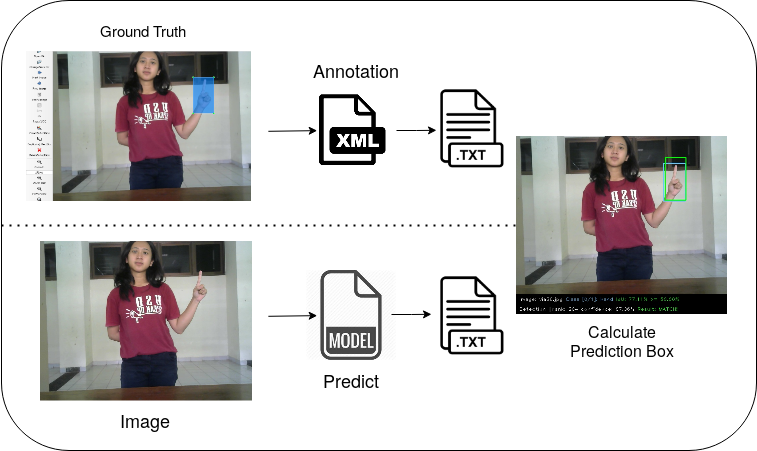
\includegraphics[width=0.8\linewidth]{calcmap}
	\caption{Visualisasi IOU pada Citra}
	\label{fig:handdetection203}
\end{figure}
Proses pengujian mAP harus mengekstrak informasi koordinat anotasi pada dataset menjadi file txt sebagai \textit{ground truth}. Proses yang sama dilakukan untuk citra testing, namun nilai koordinat diperoleh dari hasil prediksi model. Hasil dari prediksi akan disimpan koordinatnya dalam file txt sebagai \textit{prediction box}. Implementasi mAP ditunjukan pada gambar xx.
\subsection{Kfold Cross Validation}
Model CNN yang dilatih menggunakan Kfold Cross Validation dengan k = 5, dari hasil seluruh fold dipilih model dengan nilai akurasi terbesar. Berdasarkan tabel 5.1 maka model yang akan digunakan untuk pengujian adalah model dengan dengan nilai akurasi 0.9531863 pada fold empat. Hasil dari proses pelatihan ditunjukan pada Tabel 5.1.
\begin{table}[H]
	\caption{Akurasi 5-fold Cross Validation}
	\vspace{0cm}
	\centering
	\begin{tabular}{|c|c|c|c|c|}
		\hline K=1 &  K=2 &K=3 & K=4 &K=5\\
		\hline  0.9490& 0.9399 & 0.9436& 0.9531 &0.9375 \\
		\hline
	\end{tabular}
\end{table}

\section{Implementasi Pengujian}
Implementasi pengujian pada rancangan penelitian ini meliputi pengenalan gestur tangan dan deteksi objek yang masing masing menggunakan retinex. Setelah dilakukan pengujian, peneliti melakukan pengujian yang sama namun tanpa menggunakan retinex, kemudian membandingkan hasil keduanya untuk dianalisa.
\subsection{Pengujian Pengenalan Gestur Tangan}
Pengujian pengenalan gestur tangan dilakukan seperti rancangan sistem, pada tahap ini video akan di tulis ulang untuk dianalisis ketika menggunakan Retinex dan saat sistem berjalan tanpa Retinex. Keluaran dari pengenalan gestur ini menampilkan angka yang akan dikenali oleh sistem. Implementasi program disajikan pada gambar 5.16.
\begin{figure}[H]
	\centering
	\lstinputlisting[language=python,firstline=11,lastline=23]{write_p_retinex_cnn.py}
\end{figure}
\begin{figure}[H]
	\centering
	\lstinputlisting[language=python,firstline=24,lastline=51,firstnumber=14]{write_p_retinex_cnn.py}
	\caption{Source Code Pengenalan Gestur}
\end{figure}
\subsection{Pengujian Deteksi Objek}
Proses pengujian deteksi objek dilakukan hal yang sama seperti pengujian gestur. Keluaran dari deteksi objek ini menampilkan \textit{bounding box} dari objek yang terdeteksi. Gambar 5.17 merupakan implementasi program deteksi objek. Line 6 pada program dilakukan untuk melakukan \textit{load} label untuk objek, dimana label\_map.pbtxt berisi \textit{hand} dengan id sama dengan 1. Line 8 digunakan untuk memuat model hasil pelatihan deteksi objek yang disimpan dengan nama \textit{saved\_model.pb}.
\begin{figure}[H]
	\centering
	\lstinputlisting[language=python,firstline=9,lastline=18]{with_ret.py}
\end{figure}
\begin{figure}[H]
	\centering
	\lstinputlisting[language=python,firstline=53,lastline=85,firstnumber=11]{with_ret.py}
	\caption{Source Code Deteksi Objek}
\end{figure}
\subsection{Pengujian Sistem Secara Keseluruhan}
Pengujian ketiga merupakan gabungan antara deteksi tangan dan pengenalan gestur. Keluaran dari program ini akan menampilkan objek yang terdeteksi kemudian objek tersebut akan dikenali gesturnya. Pengujaan ini dilakukan sama seperti sebelumnya. Implementasi program ditampilkan pada gambar 5.18
\begin{figure}[H]
	\centering
	\lstinputlisting[language=python,firstline=12,lastline=29]{save_sistem_keseluruhan.py}
\end{figure}
\begin{figure}[H]
	\centering
	\lstinputlisting[language=python,firstline=62,lastline=89,firstnumber=62]{save_sistem_keseluruhan.py}
\end{figure}
\begin{figure}[H]
	\centering
	\lstinputlisting[language=python,firstline=90,lastline=103,firstnumber=90]{save_sistem_keseluruhan.py}
	\caption{Source Code Sistem Keseluruhan}
\end{figure}